The study of facial gestures has acquired an increasing interest since it has a huge application area. Facial gestures can be defined as a movement produced in the face by muscles while contracting (see Figure \ref{fig:Facial muscles}) with the objective to transmit thoughts or emotions, for example when a person communicates with others. The interpretation of non-verbal human communication, like facial gesticulation during a talk, is a very common activity and is done intrinsically. Equally important is the interpretation of gestures, through this, people can improve their interpersonal understanding. For example, by analyzing the mood of a speaker it is possible to confirm the intention of a message.

\begin{figure}[ht]
\centering
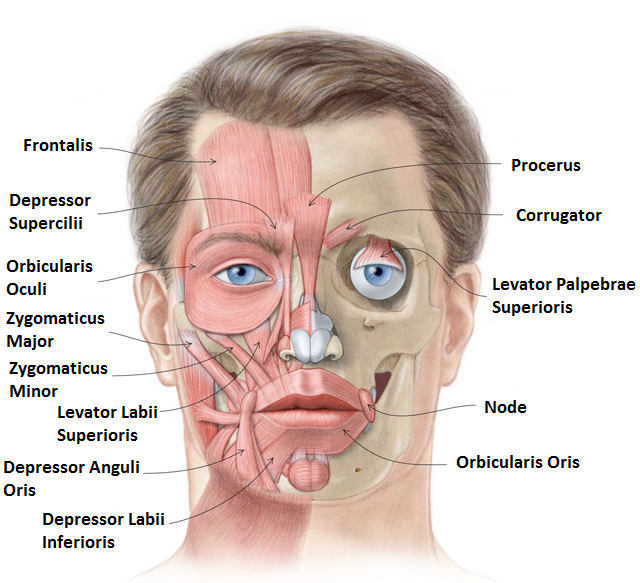
\includegraphics[scale=0.5]{images/Figure11FacialMuscles_name_2.png}
\caption{Facial muscles}
\label{fig:Facial muscles}
\end{figure}

Traditionally, computational applications have tried to interpret emotion by associating a facial image to one of the seven general expressions (such as fear, anger, happiness, etc) but they are too general and they do not evaluate the symmetry of the emotion. This can be solved considering the psychological perspective of the emotions. According to Ekman \cite{Hager1979} the symmetry of a gesticulation can describe the veracity of a expression. The bases for this are some studies of the amygdala~\cite{Sergerie2008}, which is a region in the brain (located in the medial temporal lobes) that performs the analysis of expressions.

However, this task is complex, since involves temporal processing of muscles contractions. To approach this problem, one can look at biological systems that perform this analysis accurately. An example of this is the human brain, which can perform the analysis even under varying environment conditions like: illumination changes, occlusion and pose changes. This is a motivation for the developing of bio-inspired systems based on the behavior of the amygdala, more precisely modeling the neuron interaction for analysis facial motion produced by the gestures.

From all the involved parts gesture eye gaze is the most important element since it express sincerity and credibility. Together, all the elements of the facial muscles can transmit the feelings of the speaker, from happiness, to depth concern. This was previously affirmed by Darwin~\cite{Darwin1872}, who stated that facial gesticulation for emotion transmition is innate and very similar for all people, since we evolved very similarly. His theory was not accepted before due to some detractors like Bruner et al.~\cite{Bruner1954}. Later, Ekman et al. \cite{Hager1979} solved this issue definitively by pointing out methodological problems that had confused other researchers. They showed that observers could agree on how to label both posed and spontaneous facial expressions in terms of either emotional categories or emotional dimensions. Much evidence, including reanalysis of negative studies, indicated that facial expressions can provide accurate information about emotion.

Therefore the analysis of facial expressions constitutes a critical and complex portion of our non-verbal social interactions. Over the past years there has been an increasing interest on developing automated computational tools for facial expression analysis.

\begin{comment}
However, the automatic facial expression analysis is a complex task, on one hand face structure distribution is different from one individual to another. On the other, faces are analyzed from sequences of images captured in environments with variations (such as lighting, pose and scale changes) that difficult the extraction of this structure. From the computational point of view, this problem implies the classification of facial motion and facial structure deformation into abstract representations completely based on visual information.
\end{comment}

To address this analysis it is necessary to perform two main tasks: face acquisition and facial feature extraction. In the first one, techniques have been developed to deal with the extraction and normalization of the face, considering variations in the pose %\cite{Essa1997, Rowley1998}
and illumination. %\cite{Fellenz1999, Belhumeur1997}.
However, most of the effort has been focused on the feature extraction issue~\cite{Fasel2003}, since techniques like appearance-based model %\cite{Lanitis1997, Kim2004, RuizdelSolar2008}
try to deal with significant variations in the acquired face images without relying on normalization.

\begin{figure}[ht]
    \centering
    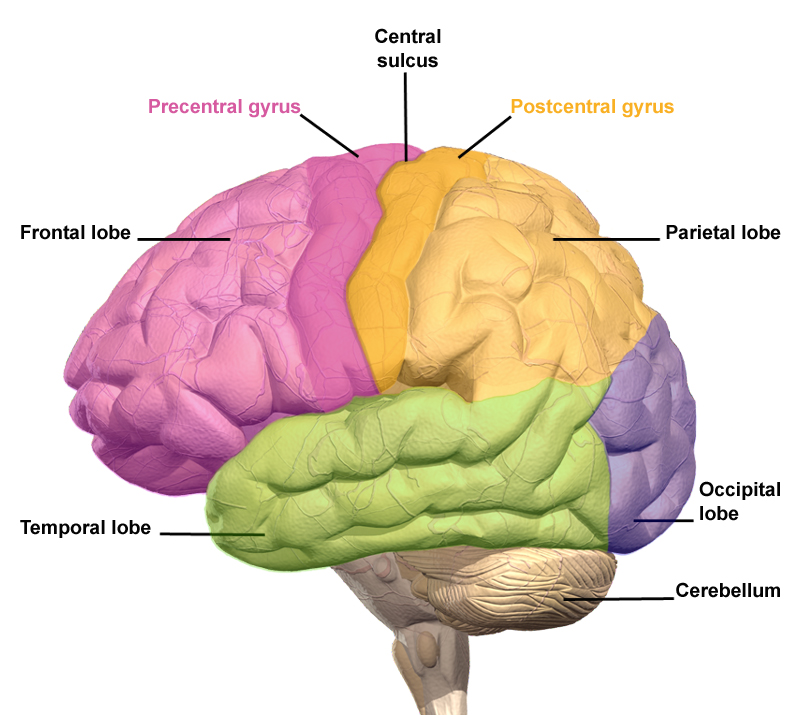
\includegraphics[scale=1.0]{images/Figure6Brain.png}
    \caption{Brain anatomy}
    \label{fig:Brain anatomy}
\end{figure}

The analysis problem has been approached from two main streams~\cite{Fasel2003}: facial deformation extraction models and facial motion extraction models. Motion extraction approaches directly focus on facial changes produced by facial expressions, whereas deformation-based methods contrast the visual information against face models to extract features product of expressions and not by age deformation like wrinkles.

\begin{comment}
In the case of deformation methods the extraction of features relies on shape and texture changes through a period of time. On one hand the holistic approaches either use the whole face \cite{JyostnaDevi2010}%, Nair2011}
or partial information about regions in the face like mouth or eyes \cite{Gu2012}.%, Venkatesh2009, Maalej2011}.
In the case of the motion extraction, the features are extracted by analyzing motion vectors, again this can be done holistically %\cite{Dornaika2011, Sanchez2011}
, and locally.%\cite{Park2009, Xiang2008, Wang2009}.
\end{comment}

Another approach to solve this problem, is by looking at biological systems that perform accurately this task. The human brain can analyze the information from the face using an area called amygdala which receives connections from other areas like visual cortex. How exactly the amygdala works remains unknown; however, it is know that this area sends impulses to the hypothalamus for activation of the sympathetic nervous system, to the thalamic reticular nucleus for increased reflexes, to the nuclei of the trigeminal nerve and the facial nerve, and to the ventral tegmental area, locus coeruleus, and laterodorsal tegmental nucleus for activation of dopamine, norepinephrine and epinephrine.% \cite{Amunts2005}.

The cortical nucleus is involved in the sense of smell and pheromone-processing. It receives input from the olfactory bulb and olfactory cortex. The lateral amygdala, which send impulses to the rest of the basolateral complexes and to the centromedial nuclei, receive input from the sensory systems. The centromedial nuclei are the main outputs for the basolateral complexes, and are involved in emotional arousal in rats and cats. Several studies confirm that the amygdala receives inputs from visual cortex when it comes to emotion processing. Lateralization of processing visual information in the amygdala might indicate symmetry analysis activity which was first found by Ekman et al \cite{Hager1979}. In their studies they found that emotion understanding is directly related to symmetrical analysis of opposed facial regions.

This information is relevant since provides hints on the role of the amygdala during the expression of emotions and visual interpretation of them. How the visual information is processed remains unclear, but it is known that the information is processed laterally (information is processed in one hemisphere). This can be used as a source of inspiration to build a neural architecture that allows processing opposed facial regions to interpretate emotions. Previously some researchers have used traditional neural networks (NN) to recognize emotions from face images\cite{Spiros2005}%, MatsuguKatsuhiko2003, MuhammadPrevost2008}
; however, NN in those works are used for recognition purposes though symmetry understanding in facial gestures requires analyzing the evolution of muscles during gesticulation rather than comparing gesture moments. This means that not all neural networks models are adequate for this task, in fact NN approaches can be classified in 3 generations, the two first are usually related to recognition tasks while the third also allows temporal information processing.

\subsubsection{Generations of Neural Networks}
Over the past hundred years, research has accumulated knowledge about the structure and function of the brain. The elementary processing units in the central nervous system are neurons which are connected to each other in an intricate pattern. Examples of this types of neurons are sketched in Figure \ref{fig:NeuronTypes} which shows a drawing by Ram\'on y Cajal, one of the pioneers of neuroscience around 1900. In his work, he distinguished several types of neurons, with different physical structures like triangular or circular. This picture gives a glimpse of the network of neurons in the cortex. In fact, cortical neurons and their connections are packed into a dense network with more than 104 cell bodies and several kilometers of ``wires'' per cubic millimeter. In all areas, however, neurons of different sizes and shapes form the basic elements. Wolfgang Maass %(Maass, 1997)%
outlined past and current artificial neural network research into three generations and made the following observations~\cite{Maass1996}.

\begin{figure}[ht]
    \centering
    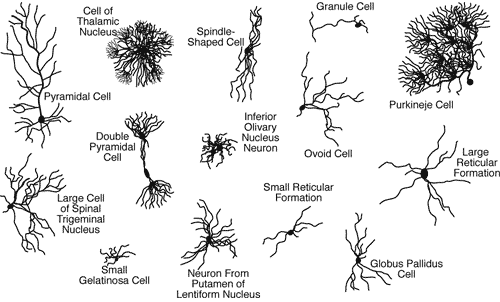
\includegraphics[scale=0.7]{images/Figure1Neuron_Types.png}
    \caption[Types of neurons]{\small{There are three kinds of neurons: motor neurons (for conveying motor information), sensory neurons (for conveying sensory information), and interneurons (which convey information between different types of neurons). The image identifies how neurons come in various shapes and sizes.}}
    \label{fig:NeuronTypes}
\end{figure}

A typical neuron can be divided into three functional parts called: dendrites, soma, and axon (see Figure \ref{fig:NeuronStructure}). Roughly speaking, the dendrites play the role of the ``input device'' that collects signals from other neurons and transmits them to the soma. The soma is the ``central processing unit'' that performs an important non-linear processing step: If the total input exceeds a certain threshold, then an output signal is generated. The output signal is taken over by the ``output device'', the axon, which delivers the signal to other neurons.

The junction between two neurons is called a synapse. Let us suppose that a neuron sends a signal across a synapse, the sender is called presynaptic cell and the receiver is called postsynaptic cell. A single neuron in vertebrate cortex often connects to more than $10^4$ postsynaptic neurons. Many of its axonal branches end in the direct neighborhood of the neuron, but the axon can also stretch over several centimeters so as to reach to neurons in other areas of the brain.

In the literature there are different computational models that intent to simulate the behavior of these neurons communities. Roughly, they can be divided in three generations, considering their chronological appearance order. Our attention is centered in the third generation since it allows temporal processing of input patterns.

The \textbf{first generation} is based on the McCulloch-Pitts neuron (also known as a perceptron or a threshold-gate) as the basic computation unit. Models of the first generation, such as the multi-layer perceptron, use digital input and output, usually binary or bipolar. The perceptron is a type of artificial neural network (ANN) invented in 1957 at the Cornell Aeronautical Laboratory by Frank Rosenblatt~\cite{Rosenblatt1960}.

The \textbf{second generation} is based on computation units (neurons) that use an activation function of a continuous set of possible output values.% Commonly, these activation functions are the sigmoid, $f(x) = 1 / 1 + e^{- \sigma x}$, or the hyperbolic tangent, $f(x) = (1 - e^{-2x}) / (1 + e^{-2x})$.
This generation, like first one, can compute arbitrary boolean functions (after using a threshold). Also, a concept of hidden layer appeared, through it more complex functions can be approximated~\cite{Rosenblatt1962}. Important to many implementations is the fact that second generation networks support learning algorithms based on gradient descent, such as error back-propagation.

\begin{figure}[ht]
    \centering
    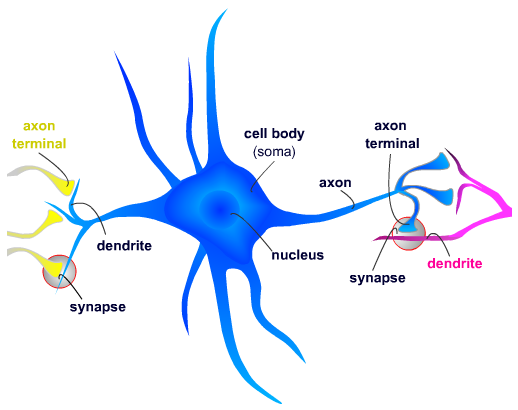
\includegraphics[scale=0.6]{images/Figure2NeuronStructure.png}
    \caption{Structure of a neuron}
    \label{fig:NeuronStructure}
\end{figure}

The \textbf{third generation} is known as Spiking Neural Networks (SNN) model. They increase the level of realism in a neural simulation, in addition to neuronal and synaptic states. The SNNs also incorporate the concept of time into their operating model, the idea is that neurons in the SNN model do not fire at each propagation cycle (as it happens with typical multi-layer perceptron networks), but rather fire only when a membrane potential\footnote{an intrinsic quality of the neuron related to its membrane electrical charge} reaches a threshold. When a neuron fires generates a signal that travels to other neurons that are stimulated (excited or inhibited) by this signal. In the context of spiking neural networks, the current activation level (modeled as some differential equation) is normally considered to be the state of the neuron, with incoming spikes pushing this value higher, and then either firing or decaying over time. Various coding methods exist for interpreting the outgoing spike train as a real-value number, either relying on the frequency of spikes, or the timing between spikes, to encode information.

\begin{figure}[ht]
    \centering
    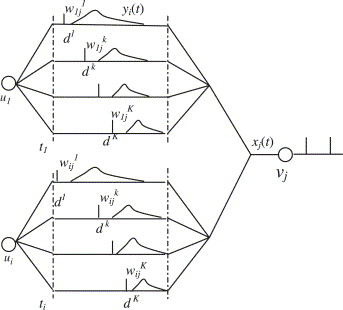
\includegraphics[scale=4.0]{images/Figure10SNN.png}
    \caption{Spiking Neural Network}
    \label{fig:Spiking Neural Network}
\end{figure}

These networks, like multi-layer perceptron networks, can approximate continuous arbitrary functions, as well as, temporal encoded inputs and outputs (\cite{Maass1996}).  This kind of neural network, in principle, can be used for information processing applications the same way as traditional artificial neural networks. However, due to their more realistic properties, they can also be used to study the operation of biological neural circuits. Some successful models of SNNs have been used to solve real-life problems, such as, navigation in mobile communities of robots \cite{WangHouZou2008}.%, BatlloriLaramee2011}. Another interesting field is sounds processing, where the SNNs have been used to detect the source of a sound \cite{NaldaCases2008}.

\begin{comment}
\subsection{SNN models}
Below there is review some widely used models of spiking and bursting neurons that can be expressed in the form of ordinary differential equations (ODE). It considers whether the models have biophysically meaningful and measurable parameters, and whether they can exhibit autonomous chaotic activity. Throughout this section, $v$ denotes the membrane potential and $v'$ denotes its derivative with respect to time. All the parameters in the models are chosen so that $v$ has $mV$ scale and the time has $ms$ scale. To compare computational cost, it is assumed that each model, written as a dynamical system $ x = f(x) $, is implemented using a fixed-step first-order Euler method $x(t+ \tau )=x(t)+ \tau f(x(t))$ with the integration time step chosen to achieve a reasonable numerical accuracy.

The models reviewed, have the computational ability of mimic various biological behaviors of neurons when they are stimulated by the incoming pulses, biological features like: excitability (tonic spiking), single spike at the onset of the input (phasic spiking), periodic bursts of spikes (tonic bursting), burst transmitting at beginning stimulation (phasic burst), bursting then spiking (mixed model), tonic spike with decreasing frequency (spike frequency adaptation) for mention a couple of them. All these characteristics of the action potential are represented, between other, by the three models which we are going to review next. Also these models have a low cost computational (number of floating point operations FLOPS).

There is a focus on three SNN models because they are very biologically plausible and they represent a low implementacion. The models are:

\begin{itemize}
\item Integrate-and-Fire-or-Burst
\item Resonate-and-Fire
\item Spiking Model by Izhikevich~\cite{Izhikevich2003}
\end{itemize}
\vspace{0.5cm}

\textbf{Integrate-and-Fire-or-Burst}\\
Smith and coauthors \cite{SmithRinzel2000} suggested an improvement integrate-and-fire-or-burst (I\&FB) to model thalamo-cortical neurons.

$$
\begin{array}{lr}
v'  =  I+a-bv+gH(v-v_h)h(v_T-v) \\
\mbox{if} \hspace{0.3cm} v  =  v_{tresh}, \hspace{0.5cm} \mbox{then} \hspace{0.2cm} v \leftarrow c \\
h'=
\left\{
\begin{array}{lr}
\frac{-h}{\tau^-}, \hspace{1cm} \mbox{if} \enspace v > v_h \\
\frac{(1-h)}{\tau^+}, \hspace{1cm} \mbox{if} \enspace v < v_h
\end{array}
\right.
\end{array}
$$

where $h$ describes the inactivation of the calcium $T$-current $g,v_h,v_T,\tau^+$ and $\tau^-$ are parameters describing dynamics of the $T$-current, and $H$ is the Heaviside step function. Having this kind of a second variable creates the possibility for bursting and other interesting regimes summarized in Table \ref{tb:ModelsComparison}. But this comes with a price: It takes between 9 and 13 operations (depending on the value of $v$) to simulate $1 ms$ of the model.

\textbf{Resonate-and-Fire}\\
The resonate-and-fire neuron \cite{Izhikevich2001} is a two-dimensional (2-D) analogue of the I\&F neuron.

$$
\begin{array}{lr}
z'=I+(b+iw)z\\
\mbox{if} \enspace Imz=a_{tresh}, \quad \mbox{then} z\leftarrow z_0(z)
\end{array}
$$

where the real part of the complex variable $z$ is the membrane potential. Here $b,w$ and $a_{tresh}$ are parameters, and $z_0(z)$ is an arbitrary function describing activity-dependent after-spike reset. The resonate-and-fire model is simple and efficient -it takes $10$ operations to simulate $1 ms$. When the frequency of oscillation $w=0$, it becomes an integrator. Its neuro-computational properties are summarized in Table \ref{tb:ModelsComparison}.

\textbf{Spiking Model by Izhikevich (2003)}\\

A simple model of spiking neurons proposed recently by Izhikevich \cite{Izhikevich2003}.

\begin{eqnarray}
\label{eq:1}
v' & = & 0.04v^2+5v+140-u+I \\
u' & = & a(bv-u)
\end{eqnarray}

with the auxiliary after-spike resetting.

\begin{eqnarray}
\label{eq:2}
\mbox{if} \enspace v \ge +30\mbox{mV}, \quad
\mbox{then}
\left\{
\begin{array}{lr}
\label{eq:3}
v \leftarrow c \\
u \leftarrow u+d
\end{array}
\right.
\end{eqnarray}

where $v$ represents the membrane potential of the neuron and $u$ represents a membrane recovery variable, which accounts for the activation of $K^+$ ionic currents and inactivation of $Na ^+ $ ionic currents, and it provides negative feedback to $v$. After the spike reaches its apex ($+30 mV$), the membrane voltage and the recovery variable are reset according to this last equation. If $v$ skips over $30$, then it first is reset to $30$, and then to $c$ so that all spikes have equal magnitudes. The part $0.04v^2+5v+140$ is chosen so that $v$ has $mV$ scale and the time has $ms$ scale. Geometrical derivation of the model based on fast and slow nullclines can be found in \cite{Izhikevich2006b}.

The model can exhibit firing patterns of all known types of cortical neurons with the choice of parameters $a$, $b$, $c$, and $d$ given in \cite{Izhikevich2003}. It takes only $13$ floating point operations to simulate $1 ms$ of the model, so it is quite efficient in large-scale simulations of cortical networks. When $(a,b,c,d)=(0.2,2,-56,-16)$ and $I=-99$, the model has chaotic spiking activity, though the integration time step $\tau$ should be small to achieve adequate numerical precision.

We stress that $+30 mV$ in equation \ref{eq:3} is not a threshold, but the peak of the spike. The threshold value of the model neuron is between $-70$ and $-50$, and it is dynamic, as in biological neurons.
\end{comment}

\subsubsection{Spiking Neural Networks}
In practice, there is a major difference between the theoretical power of spiking neural networks. Some large scale neural network models have been designed to take advantage of pulse coding found in spiking neural networks. One of the most exciting characteristics of spiking neural networks (with the potential to create a step-change in our knowledge of neural computation) is that they are innately embedded in time \cite{Maass1996}.

Spike latencies, axonal conduction delays, refractory periods, neuron resonance and network oscillations all give rise to an intrinsic ability to process time-varying data in a more natural and computationally powerful way than is available to 2nd generation models. Real brains are embedded in a time-varying environment; almost all real-world data and human or animal mental processing has a temporal dimension. Evidence is growing that rhythmic brain oscillations are strongly connected to cognitive processing.% \cite{Klimesch1999, Basar2001, Engel2001, Kahana2001, Ward2003}.
This type of processing is well suited to problems like face gesticulation characterization, since this problem implies the processing of spatial features over time periods to abstract their relations over time.

\begin{figure}[h]
    \centering
   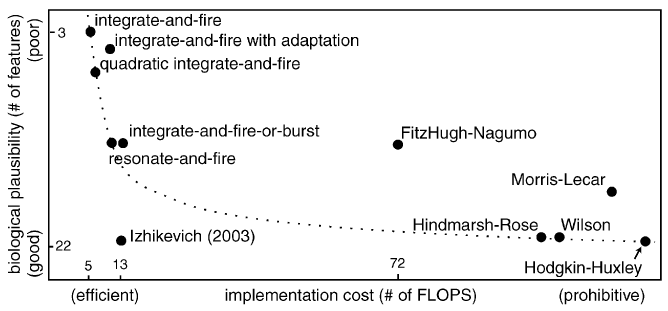
\includegraphics[scale=0.7]{images/Figure3Comparison.png}
    \caption{Comparison of spiking models: biological plausibility against implementation cost.}
    \label{fig:Comparison}
\end{figure}

\begin{comment}
\begin{table}[h]
\scriptsize
%\footnotesize
\begin{center}
\begin{tabular}{|p{3.0cm}|p{0.1cm}|p{0.1cm}|p{0.1cm}|p{0.1cm}|p{0.1cm}|p{0.1cm}|p{0.1cm}|p{0.1cm}|p{0.1cm}|p{0.1cm}|p{0.1cm}|p{0.1cm}|p{0.1cm}|p{0.1cm}|p{0.1cm}|p{0.1cm}|p{0.1cm}|p{0.1cm}|p{0.1cm}|p{0.1cm}|p{0.1cm}|p{0.1cm}|p{0.4cm}|} \hline \hline
\bf Models &
\multicolumn{1}{c|}
{\begin{sideways}
biophysically meaningful \
\end{sideways}} &
{\begin{sideways}
tonic spiking \
\end{sideways}} &
{}{\begin{sideways}
phasic spiking \
\end{sideways}} &
{}{\begin{sideways}
tonic bursting \
\end{sideways}} &
{}{\begin{sideways}
phasic bursting \
\end{sideways}} &
{}{\begin{sideways}
mixed mode \
\end{sideways}} &
{}{\begin{sideways}
spike frequency adaptation \
\end{sideways}} &
{}{\begin{sideways}
class 1 excitable \
\end{sideways}} &
{}{\begin{sideways}
class 2 excitable \
\end{sideways}} &
{}{\begin{sideways}
spike latency \
\end{sideways}} &
{}{\begin{sideways}
subthreshold oscillation \
\end{sideways}} &
{}{\begin{sideways}
resonator \
\end{sideways}} &
{}{\begin{sideways}
integrator \
\end{sideways}} &
{}{\begin{sideways}
rebound spike \
\end{sideways}} &
{}{\begin{sideways}
rebound burst \
\end{sideways}} &
{}{\begin{sideways}
threshold variability \
\end{sideways}} &
{}{\begin{sideways}
bistability \
\end{sideways}} &
{}{\begin{sideways}
DAP \
\end{sideways}} &
{}{\begin{sideways}
accomodation \
\end{sideways}} &
{}{\begin{sideways}
inhibition-indiced spiking \
\end{sideways}} &
{}{\begin{sideways}
inhibition-induced bursting \
\end{sideways}} &
{}{\begin{sideways}
chaos \
\end{sideways}} &
{}{\begin{sideways}
$\sharp$ of FLOOPS \
\end{sideways}} \\  \hline \hline
\bf integrate-and-fire &  & $\bullet$  &   &  &  &  &  & $\bullet$ &  &  &  &  & $\bullet$ &   &  &  &  &  &  &  &  &  & 5 \\  \hline \hline
\bf integrate-and-fire with adaptation &  & $\bullet$ &  &  &  &  & $\bullet$ & $\bullet$ &  &  &  &  & $\bullet$ &  &  &  &  & $\bullet$ &  &  &  &  & 10 \\  \hline \hline
\bf integrate-and-fire or burst &  & $\bullet$ & $\bullet$ &  & $\bullet$ &  & $\bullet$ & $\bullet$ &  &  &  &  & $\bullet$ & $\bullet$ & $\bullet$ &  & $\bullet$ & $\bullet$ &  &  &  &  & 13 \\  \hline \hline
\bf resonate-and-fire &  & $\bullet$ & $\bullet$ &  &  &  &  & $\bullet$ & $\bullet$ &  & $\bullet$ & $\bullet$ & $\bullet$ & $\bullet$ &  &  & $\bullet$ & $\bullet$ & $\bullet$ &  &  & $\bullet$ & 10 \\  \hline \hline
\bf quadratic integrate-and-fire &  & $\bullet$ &  &  &  &  &  & $\bullet$ &  & $\bullet$ &  &  & $\bullet$ &  &  & $\bullet$ & $\bullet$ &  &  &  &  &  & 7 \\  \hline \hline
\bf Izhikevich (2003) &  & $\bullet$ & $\bullet$ & $\bullet$ & $\bullet$ & $\bullet$ & $\bullet$ & $\bullet$ & $\bullet$ & $\bullet$ & $\bullet$ & $\bullet$ & $\bullet$ & $\bullet$ & $\bullet$ & $\bullet$ & $\bullet$ & $\bullet$ & $\bullet$ & $\bullet$ & $\bullet$ & $\bullet$ & 13 \\  \hline \hline
\bf FitzHugh-Nagumo &  & $\bullet$ & $\bullet$ &  &  &  &  & $\bullet$ &  & $\bullet$ & $\bullet$ & $\bullet$ &  & $\bullet$ &  & $\bullet$ & $\bullet$ &  & $\bullet$ & $\bullet$ &  & & 72 \\  \hline \hline
\bf Hindmarsh-Rose &  & $\bullet$ & $\bullet$ & $\bullet$ &  &  & $\bullet$ & $\bullet$ & $\bullet$ & $\bullet$ & $\bullet$ & $\bullet$ & $\bullet$ & $\bullet$ & $\bullet$ & $\bullet$ & $\bullet$ & $\bullet$ & $\bullet$ & $\bullet$ &  & $\bullet$ & 120 \\  \hline \hline
\bf Morris-Lecar & $\bullet$ & $\bullet$ & $\bullet$ &  &  &  &  & $\bullet$ & $\bullet$ & $\bullet$ & $\bullet$ & $\bullet$ & $\bullet$ & $\bullet$ &  & $\bullet$ & $\bullet$ &  & $\bullet$ & $\bullet$ &  &  & 600 \\  \hline \hline
\bf Wilson  &  & $\bullet$ & $\bullet$ & $\bullet$ &  &  & $\bullet$ & $\bullet$ & $\bullet$ & $\bullet$ & $\bullet$ & $\bullet$ & $\bullet$ & $\bullet$ & $\bullet$ & $\bullet$ &  & $\bullet$ & $\bullet$ &  &  &  & 180 \\  \hline \hline
\bf Hodgkin-Huxley & $\bullet$ & $\bullet$ & $\bullet$ & $\bullet$ &  &  & $\bullet$ & $\bullet$ & $\bullet$ & $\bullet$ & $\bullet$ & $\bullet$ & $\bullet$ & $\bullet$ & $\bullet$ & $\bullet$ & $\bullet$ & $\bullet$ & $\bullet$ & $\bullet$ &  & $\bullet$ & 1200 \\  \hline \hline
\end{tabular}
\end{center}
\caption{Comparison of the neuro-computational properties of spiking and bursting models \cite{Izhikevich2004}.}
\label{tb:ModelsComparison}
\end{table}
\end{comment}

In the literature there are several SNN models that have different characteristics that make them desirable for specific types of problems. According to Izhikevich \cite{Izhikevich2004}, to define the model that will be used to interpret facial motion it is necessary to consider two aspects about the selected SNN: biological plausibility, and computational time cost. A comparison between several SNN models is presented in Figure \ref{fig:Comparison}, where the zero shows those models means with the highest efficiency in terms of computational viability.% Considering this information, the selected models for these thesis are: Integrate and Fire or Burst and Resonate and Fire and Izhikevich. In the following we describe the basic functioning of these models.\\

%\begin{figure}[H]
  %  \centering
    %\includegraphics[scale=0.8]{Figure4ModelsPropertiesComparison.png}
    %\caption{Comparison of the neuro-computational properties of spiking and bursting models.}
    %\label{fig:ModelsPropertiesComparison}
%\end{figure}

%Linking part with Web services and image compression techniques
The gesture analysis methods, traditionally, can be used in situations like job interviews or business meetings where participants are in the same place, however, nowadays these events are carried out online, thereby decreasing the perception of those involved. Therefore arises the need of a tool or architecture that allows the use of gesture analysis methods online, but this task is not trivial, because it requires mechanisms for exchanging data between the client and the server. This issue could be solved by the use of web services, a technology that has been used for streaming video and audio.

However, given the characteristics of Internet services in the country, the transfer of information would not be very optimal, therefore a technique that allows the compression of images without loss of quality, is needed, in order to be able to perform the gesture analysis more efficiently.
